\documentclass{article}
\usepackage{indentfirst}
\usepackage[backend=biber]{biblatex}
\usepackage{graphicx}
\addbibresource{bibliografia.bib}
\usepackage{caption}
\captionsetup{
    justification=raggedright,singlelinecheck=false, labelfont=bf
}
\usepackage{hyperref}
\hypersetup{
    urlcolor=blue,
    colorlinks=true,
    citecolor=blue
}
\usepackage[spanish]{babel}



\author{Franco Ganga}
\title{Proyecto\ RUDA:\ Registro\ unificado\ de\ actividades}

\def\signed #1{{\leavevmode\unskip\nobreak\hfil\penalty50\hskip2em
  \hbox{}\nobreak\hfil(#1)%
  \parfillskip=0pt \finalhyphendemerits=0 \endgraf}}

\newsavebox\mybox
\newenvironment{aquote}[1]
  {\savebox\mybox{#1}\begin{quote}}
  {\signed{\usebox\mybox}\end{quote}}


\setlength{\parindent}{0.75cm}



\renewcommand{\figurename}{Imagen}

\begin{document}
\maketitle

\section{Introduccion}%
\label{sec:introduccion}

\subsection{Resumen}%
\label{sub:resumen}

El presente trabajo expondrá el desarrollo de un proyecto a realizarse en la Universidad Nacional Arturo Jauretche, el cual
consistirá en la elaboración de un sistema informático para el registro de datos\@. El mismo tendrá como finalidad la consolidación
de conocimientos adoptados en la carrera y requerirá de la capacidad de análisis e investigación para adaptarse a los estándares
y herramientas utilizadas por la Dirección de informática de la institución.

\subsection{Objetivos}%
\label{sub:objetivos}


El objetivo general de este proyecto es el desarrollo de un sistema que permita el registro de datos sobre las actividades
realizadas por los integrantes de la institución. El mismo almacenará datos de proyectos de investigación, publicaciones, voluntariados, etc.

Actualmente la universidad no cuenta con una plataforma establecida para el registro de esta información, sólo se dispone de
los datos de las personas que integran la institución. Estos datos están distribuidos en dos sistemas:
\begin{itemize}
    \item \textbf{SIU-Mapuche:} Sistema de RRHH de la Universidad, cuenta con toda la información relevante al personal (docente
        y no-docente) y a los cargos.
    \item \textbf{SIU-Guaraní:} Sistema Académico de la Universidad, aquí es donde se encuentran los datos de alumnos, institutos
        , materias, comisiones, carreras, etc.
\end{itemize}

El uso de estos sistemas como fuente de información, y su integración con la plataforma RUDA, permitirá saber en qué actividades
está o estuvo involucrada determinada persona en la institución. Se desarrollará una interfaz web para el acceso a los datos
, para lo cual será necesario poder relacionar la información en los sistemas fuente con la de RUDA\@. Además, se implementará
un servicio REST, que permitirá acceder fácilmente a los datos.

Este proyecto está pensado para ser utilizado por las siguientes áreas:
\begin{itemize}
    \item Centro de Política Educativa
    \item Centro de Política y Territorio
    \item Secretaría Económico Financiera
\end{itemize}


\subsubsection{Objetivos especificos}%
\label{ssub:objetivos_especificos}

Para llevar adelante el mencionado proyecto, se pretenden alcanzar los siguientes objetivos específicos:

\begin{itemize}
    \item \textbf{Modelado de datos y creación de base de datos:} Se debe modelar la estructura de los datos a almacenar en el sistema.
    \item \textbf{ABMs para interfaz de usuario:} Se Desarrollará una interfaz de usuario que permita la manipulación de los
        datos de cada actividad\@. Aquí se presentará la información de cada persona y sus actividades.
    \item \textbf{Desarrollo de la integración con los sistemas fuentes de información:} El mayor aporte a este objetivo será
        por parte del Área de sistemas de la universidad, ya que será necesario manejar información sensible.
    \item \textbf{Creación de una API REST para la obtención de los datos:} Se desarrollará un servicio web que facilite la
        manipulación de datos a través de internet. Esto brindará a la universidad la capacidad de reutilizar esta fuente de datos en futuros proyectos.
\end{itemize}

\subsection{Tareas}%
\label{sub:tareas}
A continuación, se detallarán las tareas por ejecutar en vistas al cumplimiento de los objetivos previamente definidos:

\subsubsection{Modelado conceptual de datos}%
\label{ssub:modelado_conceptual_de_datos}
Se definirá el modelado de datos a implementar basándose en los datos que se requieren almacenar y como están relacionados.

\subsubsection{Creación de la base de datos}%
\label{ssub:creación_de_la_base_de_datos}

Entidades a desarrollar que almacenarán datos  sobre la duración de cada actividad:

\begin{itemize}
    \item Cargos de Autoridad
\item Consejeros Superiores
\item Miembros y Roles en las Comisiones del Consejo Superior
\item Asambleístas
\item Consejeros Consultivos
\item Responsables de Áreas
\item Directores/Subdirectores de Institutos
\item Directores/Subdirectores de Carreras
\item Proyectos de Investigación
\item Proyectos de Extensión
\item Programas
\item Actividades de Divulgación
\item Publicaciones
\item Cursos de Extensión
\item Voluntariados
\item Vinculadores
\item Programas
\item Becas
\item Pasantías
\item Movilidad RTF
\item Movilidad Conurbano Sur
\item Prácticas Profesionales Supervisadas

\end{itemize}

\subsubsection{Definición de ABMs}%
\label{ssub:definición_de_abms}


Una ABM permite al usuario interactuar con los datos, por esto es que se deberá definir cada una en particular:

\begin{itemize}
        \item Rector
    \item Vicerrector
    \item Asambleísta
    \item Consejero Superior
    \item Responsable de Área
    \item Coordinador de Materia
    \item Miembro de Consejo Consultivo
    \item Director de Instituto
    \item Subdirector de Instituto
    \item Miembro de Comisión de Consejo Superior
    \item Director de Carrera
    \item Subdirector de Carrera
    \item Instituto
    \item Materia
    \item Carrera
    \item Consejo Consultivo
    \item Área
    \item Resolución Administrativa
    \item Comisión de Consejo Superior
    \item Rol de Comisión de Consejo Superior

\end{itemize}
\ \\No relacionadas a la política de la institución:
\begin{itemize}
        \item Práctica Profesional Supervisada
    \item Participación en Práctica Profesional Supervisada
    \item Actividad de Divulgación
    \item Curso de Extensión
    \item Participación en Curso de Extensión
    \item Pasantía
    \item Participación en Pasantía
    \item Programa
    \item Miembro de Programa
    \item Movilidad
    \item Participación en Movilidad
    \item Actividades de Vinculación
    \item Becas
    \item Participación en Beca
    \item Voluntariado
    \item Participación en Voluntariado
    \item Proyecto
    \item Miembro de Proyecto
    \item Rol de Proyecto

\end{itemize}

\subsubsection{Desarrollo de API }%
\label{ssub:desarrollo_de_api_}
Para este desarrollo se generarán rutas mediante las cuales se podrá acceder a la misma información detallada en la tarea anterior.

\begin{itemize}
    \item \textbf{Implementación de nodos para obtener cada dato:} cada dato debe ser accesible mediante una petición http.
    \item \textbf{Implementación de autenticación del servicio}
\end{itemize}

\subsubsection{Instalación y configuración de librerias}%
\label{ssub:instalación_y_configuración_de_librerias}
Se deberá configurar cada librería de acuerdo a las necesidades del sistema.
A continuación se listan las librerías a utilizar para el desarrollo:

\begin{itemize}
    \item Sonata-admin
\item Sonata-user
\item FOSUser
\item Doctrine
\item Data-Fixtures
\item Faker
\item Api-Platform

\end{itemize}

\section{Desarrollo}%
\label{sec:desarrollo}

\subsection{Aporte al proyecto}%
\label{ssub:aporte_al_proyecto}
Este proyecto se desarrolló en conjunto con otros alumnos de la universidad, por lo tanto a continuación se lista mi aporte:

\begin{itemize}
    \item Modelado de datos:
    \begin{itemize}
        \item Entidad de Consejero Superior
        \item Entidad de Miembros de proyectos
        \item Implementación de herencia en proyectos
        \item Entidad de Proyectos
        \item Entidad de Roles de Proyecto
        \item Entidad de Práctica Profesional Supervisada
        \item Entidad de Comisión de Comisión de Consejo Superior
        \item Entidad de Miembros de PPS
        \item Entidad de Miembros de CCS
    \end{itemize}
    \item Clases Admin:
    \begin{itemize}
        \item Consejero Superior
        \item Miembro de Proyecto
        \item Proyecto de extensión
        \item Proyecto de investigación
        \item Rol de Proyecto
        \item Miembro de Práctica Profesional Supervisada
        \item Miembro de Comision de Consejo Superior
        \item Práctica Profesional Supervisada
        \item Comisión de Consejo Superior
    \end{itemize}
    \item Librerías:
    \begin{itemize}
        \item Sonata-User
        \item FOSUser
        \item Doctrine Fixtures
        \item Faker
        \item Sonata-Admin
        \item API-Platform
    \end{itemize}
    \item Vista personalizada de Persona
    \item Servicio de Labels o etiquetas.
\end{itemize}


\subsection{Introduccion Symfony}%
\label{ssub:introduccion_symfony}
Symfony es un \textit{framework} PHP de código abierto para desarrollar aplicaciones web. Originalmente fue concebido por la
agencia interactiva SensioLabs para el desarrollo de sitios web para sus propios clientes. Symfony se publicó en 2005 bajo
la licencia MIT Open Source y hoy se encuentra entre los principales \textit{frameworks} disponibles para el desarrollo de PHP. \textcite{symfony-def}
\begin{aquote}{Sitio web de Symfony}
Symfony es un conjunto de componentes PHP, un \textit{framework} de aplicación web, una filosofía y una comunidad, todos trabajando juntos en armonía.
\end{aquote}
Un proyecto Symfony está conformado por varios componentes que proveen funciones básicas para una aplicación web. Entender
el funcionamiento de cada uno de ellos es necesario para una buena implementación. Para el desarrollo se utilizaron los siguientes componentes de Symfony:


\begin{itemize}
    \item \textbf{Asset:} administra la generación de URL y el versionado de hojas de estilo css, archivos JavaScript e imágenes.
\item \textbf{Console:} permite crear comandos para usar en consola. Bastante útil para tareas recurrentes.
\item \textbf{Dotenv:} administra las variables de entorno de la aplicación.
\item \textbf{Expression Language:} permite utilizar expresiones dentro de archivos de configuración para obtener lógica más compleja.
\item \label{itm:flex} \textbf{Flex:} es un componente que facilita la integración de paquetes de terceros a través de lo que se denomina recetas Symfony. Estas recetas consisten en un conjunto de instrucciones automatizadas.
\item \textbf{Form:} permite crear, procesar y reutilizar formularios.
\item \textbf{Framework:} define la configuración principal del framework.
\item \textbf{Monologbundle:} integra la librería monolog con symfony para el registro de mensajes.
\item \textbf{ORM Pack:} es la librería encargada del mapeo objeto-relacional.
\item \textbf{Process:} librería utilizada para la ejecución de subprocesos. Resuelve problemas relacionados con la diferencia entre sistemas operativos y además provee una ejecución segura.
\item \textbf{Security:} componente de seguridad de Symfony. Se encarga de definir el control de acceso, sistemas de autenticación y además de establecer los proveedores de usuarios.
\item \textbf{Serializer:} paquete de Symfony que se encarga de transformar un objeto en un formato adecuado para la transmisión de datos. Ej: JSON.
\item \textbf{Swiftmailer:} permite el envío de emails a través de un servidor propio o de terceros.
\item \textbf{Translation:} permite definir textos en la aplicación para traducción al idioma local del usuario. Este proceso es comúnmente llamado internacionalización.
\item \textbf{Twig:} Motor de templates preferido por Symfony, permite renderizar contenido html de manera fácil, organizada y segura.
\item \textbf{Validator:} componente encargado de la validación de datos. Weblink: incrementa la performance de la aplicación al utilizar HTTP2 y funciones de precarga en navegadores modernos.
\item \textbf{Yaml:} se encarga de convertir archivos YAML en arrays PHP. Gran parte de la configuración de Symfony se encuentra definida en este formato.

\end{itemize}
\newpage
\subsection{Modelado}%
\label{sub:modelado}


\subsubsection{Introducción Doctrine}%
\label{ssub:introducción_doctrine}
Con Doctrine, cada objeto PHP que se requiera persistir a la base de datos, necesita estar definido en un archivo PHP que
contiene información referente a tipos de dato y relaciones entre entidades. A este archivo se lo denomina entidad.

\begin{figure}[h]
    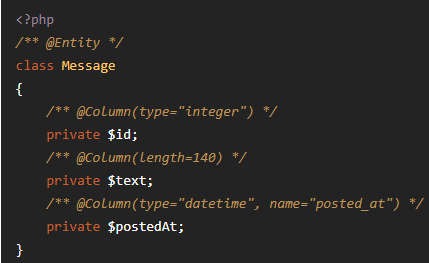
\includegraphics[width=1\linewidth]{image/entidad-doctrine.png}
    \caption{Ejemplo básico de una entidad.\newline \textbf{Fuente:} Recuperado de \href{https://www.doctrine-project.org/
    projects/doctrine-orm/en/2.6/reference/basic-mapping.html}{Documentación de Doctrine}}%
    \label{fig:image/entidad-doctrine}
\end{figure}
Una relación en \textbf{Doctrine} está formado por dos entidades. Una de ellas actúa como el lado propietario de la relación y la otra como el inverso\@.
El lado propietario de la relación es aquel en el cual \textbf{Doctrine} verifica si hubo cambios.
Existen dos tipos de mapeo de relaciones, bi-direccionales y uni-direccionales\@.
Una relación bi-direccional permite que ambos lados de la relación puedan accederse entre sí\@. En cambio, una relación uni
-direccional sólo puede accederse a través del lado propietario\@.
Al trabajar con relaciones, se debe tener en cuenta la manera en que Doctrine comprueba por cambios en los datos, ya que cambios persistidos en el lado
inverso de la relación serán ignorados por el ORM al momento de actualizar información a la base de datos.



\subsubsection{Actividad}%
\label{ssub:actividad}
Se modeló el siguiente esquema de acuerdo a la información recibida por parte del Área de informática de la universidad\@.
Además, se pensó en utilizar herencia para la definición de las actividades, de esta manera cada cargo o actividad en particular
heredaría toda característica común de una entidad padre.

\begin{figure}[h]
    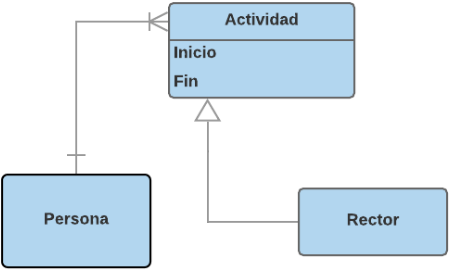
\includegraphics[scale=1]{image/actividad-modelo.png}
    \caption{Ejemplo de la definición de un cargo\newline \textbf{Fuente:} Elaboración propia}%
    \label{fig:image/actividad-modelo}
\end{figure}
El primer paso realizado para la definición de cada cargo o actividad fue la creación de la entidad Actividad, la cual contendrá
datos de la persona relacionada y el periodo de desarrollo de la actividad o cargo\@.
Se agregó la función de Soft delete o borrado lógico, la cual permite que, al borrar una actividad desde la aplicación web,
la misma es ocultada del usuario y no borrada de la base de datos\@. Esta función permite almacenar datos históricos del sistema\@.
Además, se agregó la función de Time stamps o etiquetas de tiempo, la cual hace posible el seguimiento de las fechas de creación
y actualización de cada actividad.


Se definió el mapeo de esta entidad en Doctrine mediante herencia de clase, una estrategia en la cual cada clase en la jerarquía es mapeada a varias tablas:
la propia y las de todas las clases padre. La tabla de una clase hija es vinculada a la del padre a través de una clave foránea.

Doctrine implementa esta estrategia a través del uso de una columna denominada discriminator en la tabla más alta en la jerarquía\@. Esta es la mejor
manera de lograr consultas polimórficas con herencia de clase\@. \textcite{doctrine-inheritance}\\
\noindent
Esta columna identifica el tipo de entidad. Por ejemplo: una
fila con un valor de ``director instituto'' significa que es una actividad del tipo DirectorInstituto\@.
Si no se provee el mapeo correspondiente, doctrine lo generará automáticamente utilizando el nombre de cada clase entidad en minúscula\@. \textcite{doctrine-inheritance}

\begin{figure}[h]
    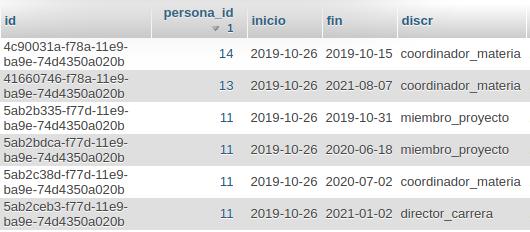
\includegraphics[width=1\linewidth]{image/discriminator-doctrine.png}
    \caption{Columna \textbf{discr} utilizada como discriminator\newline \textbf{Fuente:} Elaboración propia, impresión de pantalla del código fuente.}
    \label{fig:image/discriminator-doctrine.png}
\end{figure}
\newpage
Se agregó el la correspondiente metadata de la herencia en Actividad y se optó por proporcionar el mapeo de la columna discriminator:

\begin{figure}[h]
    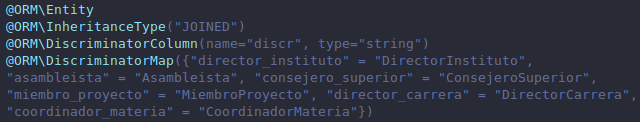
\includegraphics[width=1\linewidth]{image/discr.png}
    \caption{Mapeo de la columna \textbf{discriminator}\newline \textbf{Fuente:} Elaboración propia, impresión de pantalla del código fuente.}
    \label{fig:image/discr.png}
\end{figure}




\newpage
\printbibliography

\end{document}
